\chapter{Introdução}
Neste trabalho foi implementado um método computacional de maneira a resolver
a equação de Advecção-Difusão de forma numérica.

Para melhor entender o desenvolvimento, é necessária introdução de alguns
conceitos-chave utilizados.

\section{A Equação de Advecção-Difusão}
A equação de advecção-difusão possibilita a solução de problemas envolvendo
variações espaciais e temporais da concentração de uma substância escoando em um
fluído. Um exemplo bastante didático consiste no despejo de esgoto em um
afluente: o contaminante sofrerá efeitos difusivos --- concentrando-se ao redor
da saída --- e efeitos advectivos --- sendo carregado no sentido da correnteza.

\begin{figure}[h]
    \centering
    \captionsetup{justification=centering}
    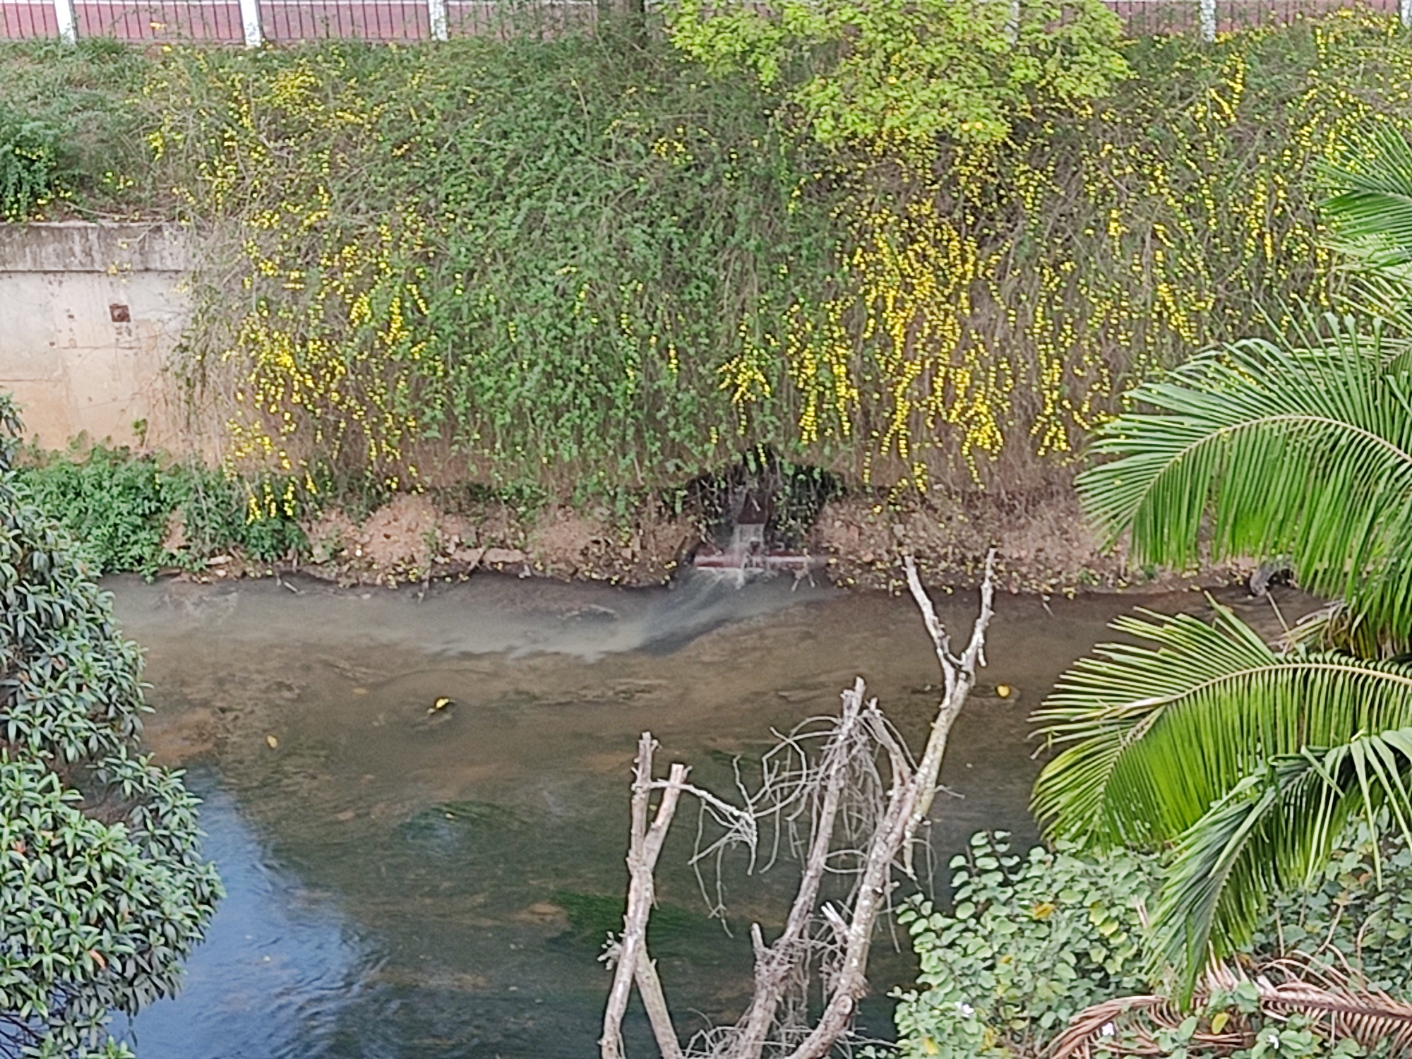
\includegraphics[width=0.7\textwidth]{esgoto}
    \caption{Efeitos difusivos e advectivos podem ser observados no despejo
    de esgoto no Rio Bengala}
\end{figure}


Para um problema unidimensional tem-se a seguinte forma,

\begin{equation}\label{adv-dif}
    \frac{\partial c}{\partial t} + \frac{\partial}{\partial x}(uc)
    - \frac{\partial}{\partial x}\left( D \frac{\partial c}{\partial x} \right)
    = 0
\end{equation}

\noindent onde $c$ indica a concentração, $u$ a velocidade e $D$ o coeficiente
de difusão.

Considerando que para $u$ e $D$ constantes, tem-se $\bar{u}$ e $\alpha$,
respectivamente, é possível reescrever Eq.\ \ref{adv-dif} como,

\begin{equation}
    \frac{\partial c}{\partial t} + \bar{u}\frac{\partial c}{\partial x} -
    \alpha\frac{\partial^2 c}{\partial x^2} = 0
\end{equation}

\section{Método dos Volumes Finitos}
O método dos volumes finitos tem como finalidade a discretização do domínio
espacial. Este é subdividido em um conjunto de volumes finitos e as variáveis
dependentes são determinadas como médias volumétricas sobre estes volumes,
avaliadas nos centros dos mesmos.

A partir da Eq.\ \ref{adv-dif}, para adaptá-la ao métodos dos volumes finitos,
é possível reescrevê-la como

\begin{equation}\label{adv-dif-volfin}
    \frac{\partial\Phi}{\partial t} + \frac{\partial f}{\partial x} = 0
\end{equation}

\noindent onde,

% Equações lado-a-lado
\noindent
\begin{minipage}{.4\linewidth}
    \begin{equation}
        \Phi = c
    \end{equation}
\end{minipage}%
\begin{minipage}{.6\linewidth}
    \begin{equation}
        f = f(c) = uc - D\frac{\partial c}{\partial x}
    \end{equation}
\end{minipage}

\bigskip
\begin{center}
    --- \textit{Inserir gráficos do domínio discretizado e explicação} ---
\end{center}
\bigskip

Para obter-se a discretização do domínio, integra-se a Eq.\ \ref{adv-dif-volfin}
no intervalo de tempo de $t^n$ a $t^{n+1}$ e no espaço de $x_{i-\frac{1}{2}}$
a $x_{i+\frac{1}{2}}$. Além disso, define-se os incrementos no tempo e no
espaço como

\begin{equation*}
    \Delta t = t^{n+1} - t^n \qquad\text{e}\qquad \Delta x = x_{i+\frac{1}{2}}
    - x_{i-\frac{1}{2}}
\end{equation*}

Tem-se, assim, uma integração dupla

\begin{equation*}
    \int_{x_{i-\frac{1}{2}}}^{x_{i+\frac{1}{2}}} \left( \int_{t^n}^{t^{n+1}}
    \frac{\partial \Phi}{\partial t}dt \right)dx
    +
    \int_{t^n}^{t^{n+1}} \left(\int_{x_{i-\frac{1}{2}}}^{x_{i+\frac{1}{2}}}
    \frac{\partial f}{\partial x}dx \right)dt
    = 0
\end{equation*}

\begin{equation}\label{int dx}
    \int_{x_{i-\frac{1}{2}}}^{x_{i+\frac{1}{2}}}[\Phi(x,t^{n+1}) -
    \Phi(x,t^n)]dx
    +
    \int_{t^n}^{t^{n+1}} [f(x_{i+\frac{1}{2}},t) - f(x_{i-\frac{1}{2}},t)]dt
    = 0
\end{equation}

Define-se uma variável $Q_i^k$ que consiste no valor médio aproximado de $\Phi$
no espaço, dado um tempo $k$ onde $k = t^n$ ou $k = t^{n+1}$

\begin{equation}\label{Qn+1}
    Q_i^n \approx \frac{1}{\Delta x}
    \int_{x_{i-\frac{1}{2}}}^{x_{i+\frac{1}{2}}} \Phi(x,t^n)dx
\end{equation}

\begin{equation}\label{Qn}
    Q_i^{n+1} \approx \frac{1}{\Delta x}
    \int_{x_{i-\frac{1}{2}}}^{x_{i+\frac{1}{2}}} \Phi(x,t^{n+1})dx
\end{equation}

Analogamente, define-se os fluxos como um $F_k^n$ que consiste no valor médio
aproximado de $F$ no tempo, dada uma posição $k$ onde $k = x_{i-\frac{1}{2}}$
ou
$k = x_{i+\frac{1}{2}}$

\begin{equation}\label{F-1/2}
    F_{i-\frac{1}{2}}^n \approx \frac{1}{\Delta t}
    \int_{t^n}^{t^{n+1}} f(x_{i-\frac{1}{2}},t)dt
\end{equation}

\begin{equation}\label{F+1/2}
    F_{i+\frac{1}{2}}^n \approx \frac{1}{\Delta t}
    \int_{t^n}^{t^{n+1}} f(x_{i+\frac{1}{2}},t)dt
\end{equation}

Substituindo as Eq.\ \ref{Qn+1}, \ref{Qn}, \ref{F-1/2} e \ref{F+1/2} na
Eq.\ \ref{int dx} e dividindo todos os termos por $\Delta x$ tem-se que

\begin{equation*}
    \frac{1}{\Delta x} \Bigg\{
    \int_{x_{i-\frac{1}{2}}}^{x_{i+\frac{1}{2}}}[\Phi(x,t^{n+1}) -
    \Phi(x,t^n)]dx
    \Bigg\}
    +
    \frac{1}{\Delta x} \Bigg\{
    \int_{t^n}^{t^{n+1}} [f(x_{i+\frac{1}{2}},t) - f(x_{i-\frac{1}{2}},t)]dt
    \Bigg\}
    = 0
\end{equation*}

\begin{equation*}
    Q_i^{n+1} - Q_i^n + \frac{1}{\Delta x} \Bigg\{
    \int_{t^n}^{t^{n+1}} [f(x_{i+\frac{1}{2}},t) - f(x_{i-\frac{1}{2}},t)]dt
    \Bigg\}
    = 0
\end{equation*}

\begin{equation*}
    Q_i^{n+1} = Q_i^n + \frac{\Delta t}{\Delta t \Delta x} \Bigg\{
    \int_{t^n}^{t^{n+1}} [f(x_{i+\frac{1}{2}},t) - f(x_{i-\frac{1}{2}},t)]dt
    \Bigg\}
\end{equation*}

Por fim, obtém-se

\begin{equation}\label{Q e F}
    Q_i^{n+1} = Q_i^n - \frac{\Delta t}{\Delta x}(F_{i+\frac{1}{2}}^n -
    F_{i-\frac{1}{2}}^n)
\end{equation}

\noindent onde o valor médio de $\Phi$ no volume de controle, $Q$, deve
ser atualizado iterativamente para o próximo passo de tempo.

Para a aproximação dos fluxos, dentre as possíveis metodologias, foi escolhido o
uso de uma aproximação \emph{upwind} para a concentração $c$:

\begin{equation}
    c \approx \frac{(Q_i^n - Q_{i-1}^n)}{\Delta x}
\end{equation}

\noindent e uma aproximação
centrada para a derivada espacial da concentração $\frac{\partial c}{\partial
x}$:

\begin{equation}
    \frac{\partial c}{\partial x} \approx \frac{(Q_{i+1}^n - 2Q_i^n +
    Q_{i-1}^n)}{\Delta x^2}
\end{equation}

\noindent que, ao serem substituídas na Eq.\ \ref{Q e F}, resultam em

\begin{equation*}
     Q_i^{n+1} = Q_i^n - \frac{\Delta t}{\Delta x} \left[
     \bar{u}Q_i^n - \alpha\frac{(Q_{i+1}^n - Q_i^n)}{\Delta x}
     - \bar{u}Q_{i-1}^n + \alpha\frac{(Q_i^n - Q_{i-1}^n)}{\Delta x}
     \right]
\end{equation*}

\begin{equation*}
    Q_i^{n+1} = Q_i^n - \frac{\Delta t}{\Delta x} \left[
    \bar{u}(Q_i^n - Q_{i-1}^n) - \alpha\frac{(Q_{i+1}^n - 2Q_i^n +
    Q_{i-1}^n)}{\Delta x}
    \right]
\end{equation*}

\begin{equation}\label{eq. final}
    Q_i^{n+1} = Q_i^n - \Delta t \left[
    \bar{u}\frac{(Q_i^n - Q_{i-1}^n)}{\Delta x} - \alpha\frac{(Q_{i+1}^n -
    2Q_i^n + Q_{i-1}^n)}{\Delta x^2}
    \right]
\end{equation}